
\chapter{Tensor Trains}
\label{chapter:tt}

An order $n$ tensor with all dimensions equal to $d$ has $d^n$ entries.
For $d=2$ and $n=50$ that is already more numbers than any computer wants to store.
The Tensor Train (TT) format~\cite{oseledets_tt} sidesteps this by writing the tensor as a chain -- a ``train'' -- of small order-3 tensors:
\[
   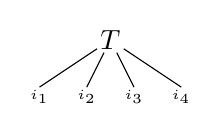
\begin{tikzpicture}[baseline=-.9em, inner sep=1pt]
      \node (T) at (0,0) {$T$};
      \draw (T) -- ++(-.9,-.6) node[pos=1, below, font=\tiny] {$i_1$};
      \draw (T) -- ++(-.3,-.6) node[pos=1, below, font=\tiny] {$i_2$};
      \draw (T) -- ++(.3,-.6) node[pos=1, below, font=\tiny] {$i_3$};
      \draw (T) -- ++(.9,-.6) node[pos=1, below, font=\tiny] {$i_4$};
   \end{tikzpicture}
   =
   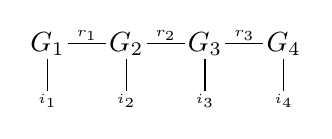
\begin{tikzpicture}[baseline=-.9em, inner sep=1pt]
      \node (G1) at (0,0) {$G_1$};
      \node (G2) at (1,0) {$G_2$};
      \node (G3) at (2,0) {$G_3$};
      \node (G4) at (3,0) {$G_4$};
      \draw (G1) -- (G2) node[midway, above, font=\tiny] {$r_1$};
      \draw (G2) -- (G3) node[midway, above, font=\tiny] {$r_2$};
      \draw (G3) -- (G4) node[midway, above, font=\tiny] {$r_3$};
      \draw (G1) -- ++(0,-.6) node[pos=1, below, font=\tiny] {$i_1$};
      \draw (G2) -- ++(0,-.6) node[pos=1, below, font=\tiny] {$i_2$};
      \draw (G3) -- ++(0,-.6) node[pos=1, below, font=\tiny] {$i_3$};
      \draw (G4) -- ++(0,-.6) node[pos=1, below, font=\tiny] {$i_4$};
   \end{tikzpicture}
   \,,
\]
or in index notation,
\[
   T_{i_1,i_2,\dots,i_n}
   = \sum_{r_1, \dots, r_{n-1}}
   (G_1)_{i_1,r_1} (G_2)_{r_1,i_2,r_2} \cdots (G_n)_{r_{n-1},i_n}
   .
\]
The tensors $G_k$ are called the \emph{cores} (or, sticking with the metaphor, the carriages) of the train.
The dangling edges $i_1,\dots,i_n$ are the original axes of $T$,
and the internal edges $r_1,\dots,r_{n-1}$ are new summation indices whose dimensions we get to choose.
The smallest dimensions $(r_1,\dots,r_{n-1})$ for which an exact representation exists are called the \emph{TT-ranks} of $T$.
If all TT-ranks are bounded by $R$, the format stores at most $n d R^2$ numbers instead of $d^n$.

In quantum physics, where the format was invented first, it is known as a \emph{Matrix Product State} (MPS)~\cite{vidal_mps, schollwock_mps}.
There the dangling edges are called ``physical'' dimensions and the internal edges ``bond'' dimensions.
The name Matrix Product State comes from the observation that each entry of $T$ is a product of matrices:
if we fix the index $i_k$ of each core, the slice $(G_k)_{:,i_k,:}$ is an $r_{k-1}\times r_k$ matrix, so
\[
   T_{i_1,\dots,i_n} = (G_1)_{i_1,:}\, (G_2)_{:,i_2,:} \cdots (G_n)_{:,i_n}
\]
is a product of a row vector, $n-2$ matrices, and a column vector,
which we can evaluate in just $O(n R^2)$ time.
This is the first hint of why the format is useful:
we never need to materialize $T$ to work with it.

Note that tensor trains generalize the two decompositions we have already seen.
For $n=2$ a tensor train is just a low-rank factorization $T = G_1 G_2$,
and the TT-rank is the matrix rank.
And if we force all internal edges to be copies of each other (contract them with a copy tensor), we recover the CP decomposition.
Compared to the Tucker decomposition of Section~\ref{sec:HOSVD}, which stores a dense $R^n$ core,
the tensor train breaks the core itself into a chain, so the storage stays linear in $n$.

\section{Cheap Operations on Trains}

The point of a compressed format is that we can compute with it directly.
Here are the most important operations.
Throughout, $T$ and $T'$ are order $n$ tensors, all of whose dimensions are $d$, given in TT format with all ranks bounded by $R$.

\paragraph{Inner products and norms.}
The inner product $\langle T, T'\rangle$ is the tensor network where all corresponding dangling edges are contracted:
\[
   \langle T, T'\rangle
   =
   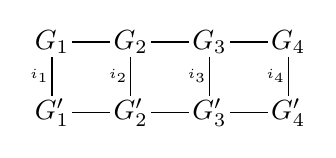
\begin{tikzpicture}[baseline=-.05em, inner sep=1pt]
      \node (G1) at (0,.45) {$G_1$};
      \node (G2) at (1,.45) {$G_2$};
      \node (G3) at (2,.45) {$G_3$};
      \node (G4) at (3,.45) {$G_4$};
      \node (H1) at (0,-.45) {$G'_1$};
      \node (H2) at (1,-.45) {$G'_2$};
      \node (H3) at (2,-.45) {$G'_3$};
      \node (H4) at (3,-.45) {$G'_4$};
      \draw (G1) -- (G2);
      \draw (G2) -- (G3);
      \draw (G3) -- (G4);
      \draw (H1) -- (H2);
      \draw (H2) -- (H3);
      \draw (H3) -- (H4);
      \draw (G1) -- (H1) node[midway, left, font=\tiny] {$i_1$};
      \draw (G2) -- (H2) node[midway, left, font=\tiny] {$i_2$};
      \draw (G3) -- (H3) node[midway, left, font=\tiny] {$i_3$};
      \draw (G4) -- (H4) node[midway, left, font=\tiny] {$i_4$};
   \end{tikzpicture}
   \,.
\]
As we saw in Section~\ref{sec:opt_contr}, the cost of evaluating such a network depends on the contraction order.
The right order here is to zip from left to right:
first contract $G_1$ with $G'_1$, giving an $R\times R$ matrix on the two bond edges;
then absorb $G_2$, then $G'_2$, and so on.
Every intermediate tensor has at most 3 edges,
and the total cost is $O(n d R^3)$.
(Contracting all the bottom row first, by comparison, would create an intermediate tensor with $n$ dangling edges -- exactly the object we are trying to avoid.)
Taking $T' = T$ gives the Frobenius norm $\|T\|_F^2$ at the same cost.

\paragraph{Sums.}
The sum $T + T'$ is again a tensor train, with ranks at most $R + R'$:
simply take the new cores to be block diagonal,
\[
   G''_k[i_k] = \begin{pmatrix} G_k[i_k] & 0 \\ 0 & G'_k[i_k]\end{pmatrix},
\]
where $G_k[i_k]$ denotes the $i_k$th matrix slice as above,
and where the first and last cores are concatenated as a row/column of blocks instead.
Multiplying the block matrices together telescopes into
$T_{i_1,\dots,i_n} + T'_{i_1,\dots,i_n}$, as promised (Exercise~\ref{ex:tt_sum}).

\paragraph{Hadamard products.}
The entry-wise product $T \circ T'$ connects each pair of dangling edges with an order-3 copy tensor, as in Section~\ref{sec:hadamard}.
Grouping each $G_k$ with $G'_k$ and the copy tensor between them gives new cores whose bond edges are the \emph{pairs} $(r_k, r'_k)$, which we can bundle with the flattening triangle from the Kronecker chapter:
\[
   \begin{tikzpicture}[baseline=-.05em, inner sep=1pt]
      \node (G2) at (1,.5) {$G_2$};
      \node (H2) at (1,-.5) {$G'_2$};
      \node[copydot] (m) at (1.35,0) {};
      \draw (G2) -- ++(-.6,0);
      \draw (G2) -- ++(.6,0);
      \draw (H2) -- ++(-.6,0);
      \draw (H2) -- ++(.6,0);
      \draw (G2) edge[bend left=25] (m);
      \draw (H2) edge[bend right=25] (m);
      \draw (m) -- ++(.5,0) node[pos=1, right, font=\tiny] {$i_2$};
   \end{tikzpicture}
   \quad\to\quad
   \begin{tikzpicture}[baseline=-.05em, inner sep=1.5pt]
      \node[triangle, rotate=180, inner sep=3pt] (l) at (0,0) {};
      \node (G2) at (1.1,.6) {$G_2$};
      \node (H2) at (1.1,-.6) {$G'_2$};
      \node[copydot] (m) at (1.7,0) {};
      \node[triangle, inner sep=3pt] (r) at (2.6,0) {};
      \draw[double] (l) -- ++(-.5,0);
      \draw (l) edge[bend left=15] (G2);
      \draw (l) edge[bend right=15] (H2);
      \draw (G2) edge[bend left=15] (r);
      \draw (H2) edge[bend right=15] (r);
      \draw[double] (r) -- ++(.5,0);
      \draw (G2) edge[bend left=20] (m);
      \draw (H2) edge[bend right=20] (m);
      \draw (m) -- ++(.55,0) node[pos=1, right, font=\tiny] {$i_2$};
   \end{tikzpicture}
   \,,
\]
so $T \circ T'$ has TT-ranks at most $R R'$.
The ranks multiply rather than add,
which is why repeated Hadamard products (say, when representing probability distributions or running many gradient steps) require periodic re-compression -- see the rounding procedure below.

\paragraph{Matrices in TT format.}
A matrix $A \in \R^{d^n \times d^n}$ can be stored as an order $2n$ tensor where core $k$ carries \emph{two} dangling edges, one row-index $i_k$ and one column-index $j_k$:
\[
   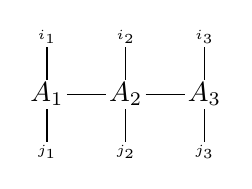
\begin{tikzpicture}[baseline=-.05em, inner sep=1pt]
      \node (A1) at (0,0) {$A_1$};
      \node (A2) at (1,0) {$A_2$};
      \node (A3) at (2,0) {$A_3$};
      \draw (A1) -- (A2);
      \draw (A2) -- (A3);
      \draw (A1) -- ++(0,.6) node[pos=1, above, font=\tiny] {$i_1$};
      \draw (A2) -- ++(0,.6) node[pos=1, above, font=\tiny] {$i_2$};
      \draw (A3) -- ++(0,.6) node[pos=1, above, font=\tiny] {$i_3$};
      \draw (A1) -- ++(0,-.6) node[pos=1, below, font=\tiny] {$j_1$};
      \draw (A2) -- ++(0,-.6) node[pos=1, below, font=\tiny] {$j_2$};
      \draw (A3) -- ++(0,-.6) node[pos=1, below, font=\tiny] {$j_3$};
   \end{tikzpicture}
   \,.
\]
This is called a TT-matrix, or in physics a \emph{Matrix Product Operator} (MPO)~\cite{oseledets_qtt}.
The product $y = Ax$ of an MPO (ranks $S$) with a tensor train $x$ (ranks $R$) is computed by stacking the two chains and contracting the shared edges;
the result is again a tensor train, with ranks at most $RS$, computable in time $O(n d^2 R^2 S^2)$.
This is the trick behind ``tensorizing'' neural networks~\cite{novikov_tensorizing}:
a $1024 \times 1024$ dense layer, reshaped as an order-20 tensor of dimensions $2$ and stored as a low-rank MPO, can use hundreds of times fewer parameters, while the matrix-vector product -- and, by the results of the derivative chapters, backpropagation -- runs directly in the compressed format.

\section{What are the TT-ranks?}

For matrices we understand rank well.
Happily, TT-ranks reduce to matrix ranks.
Cut the train between carriage $k$ and $k+1$, and let
$T_{\langle k\rangle} \in \R^{d^k \times d^{n-k}}$
denote the flattening of $T$ that bundles the first $k$ edges into a row index and the rest into a column index.

The train itself proves that $\mathrm{rank}(T_{\langle k\rangle}) \le r_k$:
everything to the left of bond $r_k$ is a $d^k \times r_k$ matrix (after flattening), everything to the right is $r_k \times d^{n-k}$, and $T_{\langle k\rangle}$ is their product:
\[
   \begin{tikzpicture}[baseline=-.05em, inner sep=1.5pt]
      \node[triangle, rotate=180, inner sep=3pt] (l) at (-1,0) {};
      \node (G1) at (0,.5) {$G_1$};
      \node (G2) at (0,-.5) {$G_2$};
      \node (G3) at (1.7,.5) {$G_3$};
      \node (G4) at (1.7,-.5) {$G_4$};
      \node[triangle, inner sep=3pt] (r) at (2.7,0) {};
      \draw[double] (l) -- ++(-.5,0);
      \draw (l) edge[bend left=15] (G1);
      \draw (l) edge[bend right=15] (G2);
      \draw (G1) -- (G2) node[midway, left, font=\tiny] {$r_1$};
      \draw (G2) -- (G3) node[pos=.5, below right=-2pt, font=\tiny] {$r_2$};
      \draw (G3) -- (G4) node[midway, right, font=\tiny] {$r_3$};
      \draw (G3) edge[bend left=15] (r);
      \draw (G4) edge[bend right=15] (r);
      \draw[double] (r) -- ++(.5,0);
   \end{tikzpicture}
\]
(Here we cut at $k=2$, redrew the chain so that carriages $1,2$ sit on the left of the bond edge $r_2$ and carriages $3,4$ on the right, and flattened both sides.)

More surprisingly, the bound is tight, so
\[
   \text{TT-rank}_k(T) = \mathrm{rank}\left(T_{\langle k\rangle}\right),
\]
and the minimum is achieved for all $k$ \emph{simultaneously} by a single train~\cite{oseledets_tt}.
We prove this constructively in the next section.

The same cut argument works for any tensor network, not just trains,
and is worth stating in general~\cite{rakhshan_cookbook}:
\emph{if a tensor $T$ is given by any tensor network, and we split its dangling edges into two groups $I$ and $J$, then the rank of the flattening $T_{(I;J)}$ is at most the product of the dimensions of the network edges crossed by any cut separating the $I$-edges from the $J$-edges.}
The network factors through the cut, just like the picture above.
For example, this immediately gives $\mathrm{rank}(AB) \le$ (dimension of the middle edge),
and it explains why networks with loops, like the PEPS grids used in physics, can represent tensors whose flattenings have exponentially large rank even when every core is small:
a cut may have to cross many edges at once.

\section{TT-SVD: Computing the Decomposition}

Unlike the CP decomposition, which is NP-hard to compute,
an exact (or optimally truncated, in the SVD sense) tensor train can be computed by a sequence of $n-1$ matrix factorizations.
The algorithm peels off one carriage at a time.
Start by flattening all but the first edge of $T$ and computing a (thin) SVD or QR factorization:
\[
   \begin{tikzpicture}[baseline=-.05em, inner sep=1pt]
      \node (T) at (0,0) {$T$};
      \node[triangle, inner sep=3pt] (r) at (1,0) {};
      \draw (T) -- ++(-.6,0) node[pos=1, left, font=\tiny] {$i_1$};
      \draw (T) edge[bend left=25] (r);
      \draw (T) edge[bend right=25] (r);
      \draw[double] (r) -- ++(.5,0);
   \end{tikzpicture}
   =
   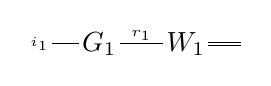
\begin{tikzpicture}[baseline=-.05em, inner sep=1pt]
      \node (Q) at (0,0) {$G_1$};
      \node (W) at (1.1,0) {$W_1$};
      \draw (Q) -- ++(-.6,0) node[pos=1, left, font=\tiny] {$i_1$};
      \draw (Q) -- (W) node[midway, above, font=\tiny] {$r_1$};
      \draw[double] (W) -- ++(.7,0);
   \end{tikzpicture}
\]
where $G_1$ has orthonormal columns (it is the $U$ of the SVD)
and $W_1 = \Sigma V^T$ is whatever remains.
Now unflatten $W_1$, group its bond edge $r_1$ together with the edge $i_2$, flatten the rest, and factor again:
\[
   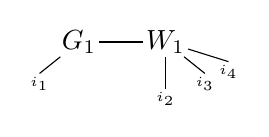
\begin{tikzpicture}[baseline=-.05em, inner sep=1pt]
      \node (Q) at (0,0) {$G_1$};
      \node (W) at (1.1,0) {$W_1$};
      \draw (Q) -- ++(-.5,-.4) node[pos=1, below, font=\tiny] {$i_1$};
      \draw (Q) -- (W);
      \draw (W) -- ++(0,-.6) node[pos=1, below, font=\tiny] {$i_2$};
      \draw (W) -- ++(.5,-.4) node[pos=1, below, font=\tiny] {$i_3$};
      \draw (W) -- ++(.8,-.25) node[pos=1, below, font=\tiny] {$i_4$};
   \end{tikzpicture}
   =
   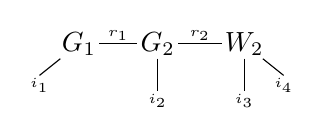
\begin{tikzpicture}[baseline=-.05em, inner sep=1pt]
      \node (Q) at (0,0) {$G_1$};
      \node (Q2) at (1,0) {$G_2$};
      \node (W) at (2.1,0) {$W_2$};
      \draw (Q) -- ++(-.5,-.4) node[pos=1, below, font=\tiny] {$i_1$};
      \draw (Q) -- (Q2) node[midway, above, font=\tiny] {$r_1$};
      \draw (Q2) -- ++(0,-.6) node[pos=1, below, font=\tiny] {$i_2$};
      \draw (Q2) -- (W) node[midway, above, font=\tiny] {$r_2$};
      \draw (W) -- ++(0,-.6) node[pos=1, below, font=\tiny] {$i_3$};
      \draw (W) -- ++(.5,-.4) node[pos=1, below, font=\tiny] {$i_4$};
   \end{tikzpicture}
   = \cdots =
   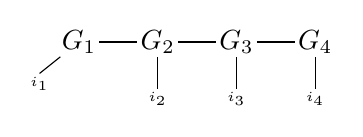
\begin{tikzpicture}[baseline=-.05em, inner sep=1pt]
      \node (Q) at (0,0) {$G_1$};
      \node (Q2) at (1,0) {$G_2$};
      \node (Q3) at (2,0) {$G_3$};
      \node (Q4) at (3,0) {$G_4$};
      \draw (Q) -- ++(-.5,-.4) node[pos=1, below, font=\tiny] {$i_1$};
      \draw (Q) -- (Q2);
      \draw (Q2) -- ++(0,-.6) node[pos=1, below, font=\tiny] {$i_2$};
      \draw (Q2) -- (Q3);
      \draw (Q3) -- ++(0,-.6) node[pos=1, below, font=\tiny] {$i_3$};
      \draw (Q3) -- (Q4);
      \draw (Q4) -- ++(0,-.6) node[pos=1, below, font=\tiny] {$i_4$};
   \end{tikzpicture}
   \,.
\]
Since each step is an exact factorization, the final train is exact,
and the rank produced at step $k$ is $\mathrm{rank}(T_{\langle k\rangle})$ -- which proves the theorem of the previous section.
If instead we \emph{truncate} each SVD, keeping only the largest singular values,
we get a low-rank approximation whose error is controlled:
truncating with error $\eps_k$ at step $k$ gives
$\|T - \widetilde T\|_F^2 \le \sum_k \eps_k^2$,
which is within a factor $\sqrt{n-1}$ of the best possible TT approximation at those ranks~\cite{oseledets_tt}.

\paragraph{Orthogonal cores.}
The cores produced by TT-SVD are special:
each $G_k$ (except the last) satisfies
\[
   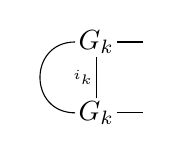
\begin{tikzpicture}[baseline=-.05em, inner sep=1pt]
      \node (A) at (0,.45) {$G_k$};
      \node (B) at (0,-.45) {$G_k$};
      \draw (A) -- (B) node[midway, left, font=\tiny] {$i_k$};
      \draw (A) edge[out=180, in=180, looseness=1.7] (B);
      \draw (A) -- ++(.6,0);
      \draw (B) -- ++(.6,0);
   \end{tikzpicture}
   \;=\;
   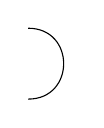
\begin{tikzpicture}[baseline=-.05em, inner sep=1pt]
      \draw (0,.45) .. controls (.6,.45) and (.6,-.45) .. (0,-.45);
   \end{tikzpicture}
   \,,
\]
that is, flattening the left bond and the dangling edge together gives a matrix with orthonormal columns.
Such cores are called \emph{left-orthogonal}.
Orthogonality is what makes the truncated SVD steps above optimal,
and it is also numerically pleasant:
if all cores but one are orthogonal (a ``canonical form'', with the remaining core called the center of orthogonality),
then the Frobenius norm of the whole train equals the norm of that single core,
and truncating there is exactly a local SVD problem.
Algorithms on trains, like the alternating least squares (ALS/DMRG) methods that optimize one core at a time~\cite{holtz_als, schollwock_mps},
sweep the center of orthogonality back and forth along the train using cheap QR factorizations.

\paragraph{Rounding.}
We saw that sums and Hadamard products increase the TT-ranks.
The fix is \emph{TT-rounding}~\cite{oseledets_tt}: given a train with inflated ranks $R'$,
sweep right-to-left making all cores right-orthogonal (QR factorizations only),
then sweep left-to-right applying truncated SVDs as in TT-SVD.
This costs $O(n d R'^3)$ -- polynomial in everything -- and is exactly equivalent to running TT-SVD on the full tensor, without ever materializing it.

\section{Quantized Tensor Trains}

Nothing stops us from applying tensor trains to plain vectors.
Take a vector $v \in \R^{2^n}$, reshape it into an order $n$ tensor of shape $2 \times 2 \times \cdots \times 2$ (index it by the bits of the original index), and decompose.
This is called the \emph{quantized} tensor train (QTT)~\cite{oseledets_qtt}.
If the TT-ranks come out bounded by $R$, we have compressed $v$ from $2^n$ numbers down to $O(n R^2)$.

Remarkably many structured vectors have tiny QTT ranks.
The geometric sequence $v_i = q^i$ has rank 1
(Exercise~\ref{ex:qtt_geometric}),
the sequences $v_i = \sin(a i + b)$ and $v_i = i$ have rank 2,
and polynomials of degree $p$ have rank $p+1$.
Structured matrices compress too, as TT-matrices on bit indices:
the identity is rank 1 (the QTT cores are copy tensors),
the tridiagonal second-difference (Laplacian) matrix has rank 3,
and the DFT matrix from the Fourier chapter has QTT ranks polylogarithmic in the accuracy $1/\eps$ after $\eps$-truncation -- the butterfly diagrams we drew there are morally a tensor train growing one carriage per FFT level.
This gives algorithms with $\log$-dimension complexity: solving a discretized PDE on $2^{50}$ grid points becomes a sequence of operations on trains of 50 tiny cores.

\section{Sketching Tensor Products}
\label{sec:tt_sketching}

We finish the chapter with a different way random compression interacts with tensor networks,
following~\cite{ahle_sketching}.
Suppose we want the rank-1 tensor
$x^{\otimes p} = x \otimes x \otimes \cdots \otimes x \in \R^{d^p}$
-- for instance because its inner products
$\langle x^{\otimes p}, y^{\otimes p}\rangle = \langle x, y\rangle^p$
compute the polynomial kernel in machine learning.
Materializing $d^p$ entries is out of the question,
so we want a random linear \emph{sketch} $\Pi \in \R^{m \times d^p}$, with small $m$, such that
$\|\Pi x^{\otimes p}\|_2 \approx \|x^{\otimes p}\|_2$
(and more generally, such that inner products are preserved).
The catch: $\Pi$ itself has $m d^p$ entries,
so $\Pi$ must \emph{itself} be a tensor network we never materialize.

\paragraph{A first attempt.}
The simplest idea is to take $p$ independent random sketch matrices $M^{(1)},\dots,M^{(p)} \in \R^{m\times d}$
and combine them row-wise, so that row $j$ of $\Pi$ is the tensor product of the $j$th rows of the $M^{(k)}$.
Row-wise combination is exactly a copy tensor on the output edge
(this is the Khatri--Rao product; compare Section~\ref{sec:hadamard}),
so the sketched vector is
\[
   \Pi x^{\otimes p}
   =
   \begin{tikzpicture}[baseline=-.05em, inner sep=1pt]
      \node[copydot] (m) at (0,0) {};
      \node (M1) at (.9,.7) {$M^{(1)}$};
      \node (M2) at (.9,0) {$M^{(2)}$};
      \node (M3) at (.9,-.7) {$M^{(3)}$};
      \node (x1) at (1.9,.7) {$x$};
      \node (x2) at (1.9,0) {$x$};
      \node (x3) at (1.9,-.7) {$x$};
      \draw (m) -- ++(-.6,0) node[pos=1, left, font=\tiny] {$j$};
      \draw (m) edge[bend left=15] (M1);
      \draw (m) -- (M2);
      \draw (m) edge[bend right=15] (M3);
      \draw (M1) -- (x1);
      \draw (M2) -- (x2);
      \draw (M3) -- (x3);
   \end{tikzpicture}
   \,,
\]
i.e.\ $(\Pi x^{\otimes p})_j = \prod_{k=1}^p (M^{(k)} x)_j$,
computable in $O(p\, m\, d)$ time -- no $d^p$ anywhere.
Unfortunately, the products of $p$ independent random variables appearing in each coordinate have heavy tails:
one can show that preserving norms requires $m$ to grow \emph{exponentially} in $p$ (roughly as $3^p$), even when each $M^{(k)}$ is a perfectly good JL matrix~\cite{ahle_sketching}.
The same exponential dependence afflicts TensorSketch~\cite{pham_pagh_tensorsketch}, the FFT-based version of this construction.

\paragraph{Recursive sketching.}
The fix of~\cite{ahle_sketching} is to build $\Pi$ as a \emph{tree} of small sketches.
Take base sketches $T_k \in \R^{m \times d}$ (one per leaf)
and $S_k \in \R^{m \times m^2}$ (one per internal node),
and sketch pairwise, recursively:
\[
   \Pi x^{\otimes 4}
   =
   \begin{tikzpicture}[baseline=-.15em, inner sep=1.5pt]
      \node (S1) at (0,0) {$S_3$};
      \node (S2) at (-1,-.8) {$S_1$};
      \node (S3) at (1,-.8) {$S_2$};
      \node[triangle, rotate=90, inner sep=3pt] (f1) at (0,-.45) {};
      \node[triangle, rotate=90, inner sep=3pt] (f2) at (-1,-1.25) {};
      \node[triangle, rotate=90, inner sep=3pt] (f3) at (1,-1.25) {};
      \node (T1) at (-1.5,-1.8) {$T_1$};
      \node (T2) at (-.5,-1.8) {$T_2$};
      \node (T3) at (.5,-1.8) {$T_3$};
      \node (T4) at (1.5,-1.8) {$T_4$};
      \node (x1) at (-1.5,-2.6) {$x$};
      \node (x2) at (-.5,-2.6) {$x$};
      \node (x3) at (.5,-2.6) {$x$};
      \node (x4) at (1.5,-2.6) {$x$};
      \draw (S1) -- ++(0,.6) node[pos=1, above, font=\tiny] {$j$};
      \draw[double] (S1) -- (f1);
      \draw (f1) edge[bend right=20] (S2);
      \draw (f1) edge[bend left=20] (S3);
      \draw[double] (S2) -- (f2);
      \draw[double] (S3) -- (f3);
      \draw (f2) edge[bend right=15] (T1);
      \draw (f2) edge[bend left=15] (T2);
      \draw (f3) edge[bend right=15] (T3);
      \draw (f3) edge[bend left=15] (T4);
      \draw (T1) -- (x1);
      \draw (T2) -- (x2);
      \draw (T3) -- (x3);
      \draw (T4) -- (x4);
   \end{tikzpicture}
\]
Reading from the bottom:
each leaf compresses one copy of $x$ to $m$ dimensions;
each internal node takes two $m$-dimensional sketches, forms (implicitly) their $m^2$-dimensional tensor product, and compresses it back to $m$ dimensions.
The whole sketching matrix $\Pi$ is a tree tensor network with $2p - 1$ random cores, each of them small.
With this construction the exponential blow-up disappears:
a target dimension $m$ that is \emph{polynomial} in $p$ and $1/\eps$ suffices,
and the analysis shows the error compounds only additively over the $O(p)$ nodes of the tree~\cite{ahle_sketching}.

Two practical notes.
First, the internal sketches $S_k$ must support fast multiplication on tensor products $u \otimes v$ \emph{without} forming the $m^2$-dimensional vector;
degree-two TensorSketch does this in $O(m \log m)$ time via the FFT,
so the full sketch takes $O(p(\mathrm{nnz}(x) + m\log m))$ time.
Second, the shape of the tree is a design choice, just like a contraction order:
a balanced tree has depth $\log_2 p$,
while a maximally unbalanced ``caterpillar'' tree -- absorb one new leaf at each level -- makes $\Pi$ literally a tensor train whose carriages are random sketches.
Random tensor networks, in other words, are not just objects we compress;
they are also the compressors.

Because the sketch is linear in $x^{\otimes p}$,
it extends beyond powers of a single vector:
it applies to any vector in $\R^{d^p}$,
and by Taylor-expanding
$e^{\langle x,y \rangle} = \sum_p \langle x,y\rangle^p / p!$
one gets sketches for the Gaussian kernel
$e^{-\|x-y\|^2/2}$
whose dimension is polynomial in the data radius and logarithmic in the accuracy -- see \cite{ahle_sketching} for details, and the Taylor material in Chapter~\ref{chapter:functions} for the diagrammatic view of such expansions.

\section{Exercises}

\begin{exercise}
\label{ex:tt_sum}
Verify the block construction for sums:
with cores $G''_k[i] = \smat{G_k[i] & 0 \\ 0 & G'_k[i]}$ for $1 < k < n$,
$G''_1[i] = \smat{G_1[i] & G'_1[i]}$ and
$G''_n[i] = \smat{G_n[i] \\ G'_n[i]}$,
show that the resulting train represents $T + T'$.
\end{exercise}

\begin{exercise}
\label{ex:qtt_geometric}
Let $v \in \R^{2^n}$ be the geometric sequence $v_i = q^i$, $i = 0, \dots, 2^n - 1$.
Show that the QTT representation of $v$ has all ranks equal to 1.
(Hint: write $i$ in binary as $i = \sum_k b_k 2^{n-k}$ and use $q^i = \prod_k (q^{2^{n-k}})^{b_k}$.)
Then show that $v_i = \sin(a i + b)$ gives ranks at most 2.
(Hint: angle addition formulas, or write $\sin$ using two complex geometric sequences.)
\end{exercise}

\begin{exercise}
Show that the order $n$ copy tensor has all TT-ranks equal to $d$,
with cores that are themselves order-3 copy tensors.
In pictures: a hyperedge connecting $n$ tensors can always be replaced by a chain of 3-way copy tensors.
\end{exercise}

\begin{exercise}
Use the cut bound to show that the TT-ranks of an order $n$ tensor satisfy
$r_k \le \min(d^k, d^{n-k})$,
and that both the all-ones tensor and, more generally, any rank-1 tensor $a_1 \otimes \cdots \otimes a_n$ has all TT-ranks 1.
\end{exercise}

\begin{exercise}
Prove diagrammatically that the first-attempt sketch satisfies
$(M^{(1)} \bullet M^{(2)})(x \otimes y) = (M^{(1)} x) \circ (M^{(2)} y)$,
where $\bullet$ is the row-wise (Khatri--Rao) product and $\circ$ the Hadamard product.
% Answer: both sides are the diagram with a copy tensor on the output edge
% joining M1x and M2y; this is the definition of Hadamard from sec:hadamard.
\end{exercise}
